\section{Implementation of a Parametric SABR Model and Implicit Neural Network Architectures}
\label{sec:implementation}

\subsection{Defining the SABR Model Equations}
\label{subsec:sabr}
The SABR model is a stochastic differential model, defined by the following equations in which the dynamics of the
asset price and the corresponding volatility levels are used to calculate an approximation to the implied volatility where no contract is traded.
\begin{itemize}
    \item \textbf{Alpha (\(\alpha\))}: This is the initial volatility level.
    \item \textbf{Beta (\(\beta\))}: The elasticity parameter between the volatility of the asset and its price.
    \item \textbf{Rho (\(\rho\))}: Statistical correlation between the asset price and its volatility, also called \textit{spot-volatility correlation}.
    \item \textbf{Volvol (\(\nu\))}: The volatility of the volatility process itself.
\end{itemize}

The simplified function for the implied volatility using the SABR model and logarithmic
``moneyness'' $x = \log\left(\frac{K}{F_t}\right)$ is then given by~\cite{Hagan2002}:
\begin{equation*}
    \sigma_{\textit{BS}}(F_t, K) =
    \alpha \frac{K^{\frac{1 - \beta}{2}}}{1 + \left( \frac{(1 - \beta)^2 \rho^2}{24} + \frac{(1 - \beta)^2(2 - 3\rho^2)}{1920} \right) (F_t K)^{1 - \beta}}\\
    \text{, where } F_t = S e^{(r - q)t}
\end{equation*}
and $S$ is the underlying asset price, $r$ is the risk-free rate, $q$ is the dividend yield, $t$ is the time to maturity,
$K$ is the strike price and $F_t$ is the forward price of the asset for a given time to maturity.
The equation presented above corresponds to the simplified version of the equation,
which does not contain all specifiable parameters.
Refer to \Cref{sec:sabr} for the full equation which is used in the actual implementation.

In our approach, we optimize one set of SABR parameters for each unique strike price per day.
Three continuous functions map from continuous maturities to the model parameters $\alpha$, $\rho$, and $\nu$.
This ensures a smooth transition between the different strike levels,
as using a single choice for the parameters for all strike and day pairs alone can introduce discontinuity in the resulting implied volatility surfaces~\citep{Hagan2015, Kim2021}.
Given the functions for the parameters $\alpha_t = f_{\alpha}(t, \textbf{P})$, $\rho_t = f_{\rho}(t, \textbf{Q})$, and $\nu_t = f_{\nu}(t, \textbf{R})$\footnote{
    The value for $\beta$ corresponds to the sensitivity of the forward price towards movements in the spot price,
    and represents a characteristic of the asset itself.
    As it does not change significantly over time to justify additional calibration,
    we treat it as a constant hyperparameter instead.
},
and the encoding variables \textbf{P, Q}, and \textbf{R} respectively,
such that $\textbf{P} \in \mathbb{R}^{5}$, $\textbf{Q} \in \mathbb{R}^{4}$, and $\textbf{R} \in \mathbb{R}^{4}$.
The functions for the parameters can then be expressed in terms of the encoding variables and continuous time to maturity $t$ as follows:

\begin{equation*}
    \label{eq:f_alpha}
    f_{\alpha}(t, \textbf{P}) = P_0 + \frac{p_3}{P_4} \left( \frac{1 - e^{-P_4 t}}{P_4 t} \right) + \frac{P_1}{P_2} e^{-P_2 t}
\end{equation*}
\begin{equation*}
    \label{eq:f_rho}
    f_{\rho}(t, \textbf{Q}) = Q_0 + Q_1 t + Q_2 e^{-Q_3 t}
\end{equation*}
\begin{equation*}
    \label{eq:f_nu}
    f_{\nu}(t, \textbf{R}) = R_0 + R_1 t^{R_2} e^{R_3 t}
\end{equation*}

Therefore, the task simply becomes obtaining the encoding variables \textbf{P}, \textbf{Q}, and \textbf{R} for each daily observed data points.
We use the Broyden-Fletcher-Goldfarb-Shanno (\textit{BFGS}) algorithm to optimize the encoding variables for minimum mean absolute error (MAE)
between the observed implied volatilities and corresponding SABR-generated implied volatilities, in other words,
we chose \textbf{P}, \textbf{Q}, and \textbf{R} which best represent the observed daily surface.
Additionally, using a Monte Carlo estimation of only a subset of the daily candidate set,
we calculate summarized values for the encoding parameters, represented by $\widetilde{\textbf{P}}$, $\widetilde{\textbf{Q}}$, and $\widetilde{\textbf{R}}$.
A more detailed explanation of the estimation process is given in \Cref{subsubsec:monte_carlo}.

To get an actual estimate of how much each of the observed data points contribute to the observed surface,
we calculate a separate MAE score, called the summarized suitability (SS) score~\citep{Kim2021} for the values
$f_{\alpha}(t, \textbf{P})$, $f_{\rho}(t, \textbf{Q})$, $f_{\nu}(t, \textbf{R})$
versus the values for $f_{\alpha}(t, \widetilde{\textbf{P}})$, $f_{\rho}(t, \widetilde{\textbf{Q}})$, and $f_{\nu}(t, \widetilde{\textbf{R}})$.

This process is similar to how a human trader would manually decide which data points were most relevant in generating the observed surface,
or rather, which data points best summarize the general shape of the surface.
Thus, knowing the SS scores facilitates can guide the removal of outliers by filtering out data points with SS scores below a certain threshold
or quantile when sorting in ascending order.
Removing outliers before fitting for the SABR model parameters is done to reduce arbitrage between market observed and interpolated option contract prices~\citep{Kim2021}.

A visual representation of a surface obtained without selecting any data points for removal and thus containing an arbitrage opportunity is shown in \Cref{fig:unfitted}.
When no selection is performed to remove outliers, the resulting SABR model can generate surfaces with clear peaks,
which can result in arbitrage opportunities if a contract where to be sold or bought for the corresponding price according to the Black-Scholes\citep{Black1973} price.
Thus, by applying a selective filtering criteria, such as the Monte Carlo SS score estimate,
we can greatly reduce arbitrage opportunities.
Additionally, if we make sure no peaks or differences between the actually SABR-generated values and observed values exist,
we can be certain no arbitrage opportunity will be present with regard to the market-observed strike and maturity pairs
To solve this problem, we use a transformer-based neural network architecture to greatly increase processing the processing
speed for the estimation of the aforementioned SS scores, while inserting implicit equilibrium layers at the output
of the network to reduce the errors the SABR generated surfaces have with respect to actual observed implied volatilities.

\begin{figure}[h]
    \begin{center}
        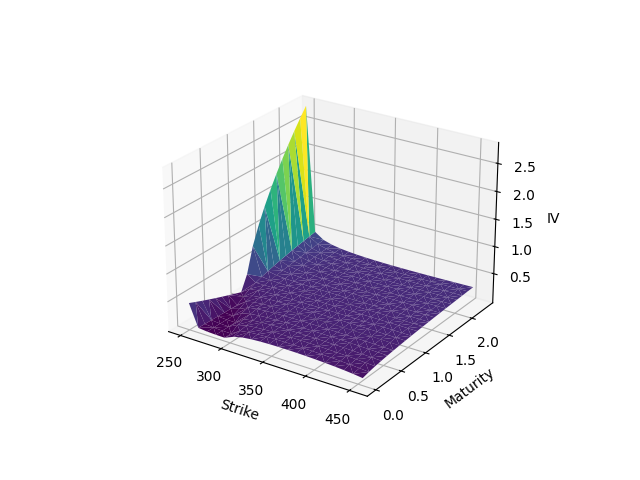
\includegraphics[width=0.55\textwidth]{images/unfitted}
        \caption{Interpolated surface using SABR models fit on a unfiltered daily candidate set.}
        \label{fig:unfitted}
    \end{center}
\end{figure}

\subsection{Proposed Architecture}
\label{subsec:architecture}

As mentioned, transformers are capable of capturing complex dependencies in sequential non-fixed length data.
Within our proposed architecture, shown in \Cref{fig:architecture}, we use a transformer encoder to approximate the \textit{SS} scores
for each candidate point $\mathcal{S}_{i}^{t} \in \mathcal{S}^{t}$ from the daily observed input.

\subsubsection{Details on the Chosen Transformer Encoder}

Unlike recurrent neural networks (RNNs) and convolutional neural networks (CNNs),
transformers do not rely on a fixed-length data sequence or fixed window size~\citep{Wen2023}.
Instead, they use an attention mechanism, which allows each input element (or token) to consider the relationship
with all other elements in the same sequence simultaneously~\citep{Vaswani2023}.
This is achieved through a block of layers using attention heads.

The attention mechanism accepts continuous data and calculates a value for different heads through the
value ($V$), key ($K$), and query ($Q$) matrices,
resulting in an output weighted by the importance of each element in the sequence.
Specifically, for our problem we use the mechanism of self-attention, and therefore the three matrices are equal.
\begin{equation}
    \label{eq:attention}
    \textit{Attention}(Q, K, V) = \textit{softmax}\left(\frac{QK^T}{\sqrt{d_k}}\right)V
\end{equation}

Transformers are classified as machine learning algorithms due to their ability to learn patterns and relationships from data,
and were originally proposed for natural language processing tasks.
In the context of our specific architecture, we use only the encoder block and adapt it to perform a regression on the SS scores.
The hidden values are passed to fully-connected (FC) layers, and implicit fixed-point iteration layers are added as final output layers.

\subsubsection{Details on the Implicit Layer}
Using a Deep Equilibrium Model variation for the Implicit Layer, we adapt \Cref{eq:fixed_point}
by using the following fixed point equation instead,
where $g$ is the MAE between the observed surface and the generated surface using the SABR model optimized on the filtered candidate set.
\begin{equation}
    \label{eq:dem}
    \begin{aligned}
        g_{\mathbf{W}}(x, z^\ast) = 0\\
        z^\ast = f(z^\ast, x)
    \end{aligned}
\end{equation}
where \textbf{W} are the layer weights and biases, $f$ is an activation function, and $z*$ is the target output of a batched non-normalized Jacobian to be used as the gradient function in our code, given by the equation below.
Finally, $y$ are the hidden values as well as the final output scores.
\[
    \left( \frac{\partial z^\ast(\cdot)}{\partial (\cdot)} \right)^T y = \left( \frac{\partial f(z^\ast, x)}{\partial (\cdot)} \right)^T g_{\mathbf{W}}
\]

\begin{figure}[h]
    \begin{center}
        
\includegraphics[width=0.8\textwidth]{images/architecture}
        \caption{Visualization of the Transformer Encoder and Implicit Layers used in the proposed architecture.}
        \label{fig:architecture}
    \end{center}
\end{figure}

\subsubsection{Monte Carlo Estimation of SS Scores}
\label{subsubsec:monte_carlo}

As mentioned in \Cref{subsec:sabr}, a Monte Carlo process is used to estimate synthetic target SS scores for the model.
Instead of using the entire daily candidate set for calculating the encoded variables \textbf{P}, \textbf{Q}, and \textbf{R} for the SABR model,
only $k$ subsets with size $p \cdot n$, where $n$ is the total number of candidate points and $p$ is a percentage value,
of the candidate set are used as input to the \textit{BFGS} algorithm to reduce surface volatility,
resulting in $\widetilde{\textbf{P}}$, $\widetilde{\textbf{Q}}$, and $\widetilde{\textbf{R}}$.
The SS score is then calculated as the mean absolute error (MAE) between the functions $f_{\alpha}$, $f_{\rho}$, and $f_{\nu}$
using both encoded variable types as shown in \Cref{alg:mc} and its normalized values are used as target values for our model.
The choice of using a neural network approach for calculating the SS scores is motivated by the much higher computational cost of the Monte Carlo estimation.

The Monte Carlo estimation is performed with a small finite number of subsets due to computational constraints, both in terms of time and memory.
Finally, model training is performed until convergence to low RMSE values between the scores predicted
with the network and the ones generated by the Monte Carlo estimation.
After training, the model prediction substitutes the Monte Carlo estimation for the SS scores,
and the best candidate set is selected and passed to the \textit{BFGS}
algorithm to obtain the final encoding $\textbf{P}_{\text{nn}}, \textbf{Q}_{\text{nn}}, \textbf{R}_{\text{nn}}$
variables for the SABR models to be used for the actual surface interpolation.

\begin{algorithm}
    \begin{algorithmic}[1]
        \Require Daily candidate set $\mathcal{S}^{t}$, percentage $p=0.8$, number of subsets $k=1 \times 10^2$
        \State $\alpha^{*}, \rho^{*}, \nu^{*} \gets \textit{BFGS} (\mathcal{S}^{t})$
        \State $\text{SS}_{\alpha}, \text{SS}_{\rho}, \text{SS}_{\nu} \gets \mathbf{0}$
        \For{candidate $c$ in $\mathcal{S}^{t}$}
            \State $\mathcal{S}_{i}^{t} \gets$ Sample($\mathcal{S}^{t}$, $k$, $p$)
            \State $\widetilde{\textbf{P}}, \widetilde{\textbf{Q}}, \widetilde{\textbf{R}} \gets \textit{BFGS}(\mathcal{S}_{i}^{t})$
            \State $\text{SS}_{\alpha, c} \gets \text{MAE}(f_{\alpha}(t, \widetilde{\textbf{P}}) - \alpha^{*})$
            \State $\text{SS}_{\rho, c} \gets \text{MAE}(f_{\rho}(t, \widetilde{\textbf{Q}}) - \rho^{*})$
            \State $\text{SS}_{\nu, c} \gets \text{MAE}(f_{\nu}(t, \widetilde{\textbf{R}}) - \nu^{*})$
        \EndFor
        \State z-normalize $\text{SS}_{\alpha}, \text{SS}_{\rho}, \text{SS}_{\nu}$
    \end{algorithmic}
    \caption{Monte Carlo Estimation of normalized Target SS Scores}
    \label{alg:mc}
\end{algorithm}
